\chapter{Resultats}
\label{c:Resultats}
\fbox{\emph{\textbf{\parbox{0.9\linewidth}{
Hem de tenir en compte de que les notes finals dels alumnes estan arrodonides, per tant considerarem que la predicció ha estat encertada si té un marge d'error menor a 0,5.}}}}
\section{Resultats de la xarxa neuronal en fulls de càlculs}
Desprès de finalitzar totes les etapes, els pesos s'han ajustat correctament i, encara que l'error no s'hagi pogut aproximar-se molt al zero absolut, ja és un valor molt petit que podem donar per bo. En la seguent figura podem veure els valors dels pesos finals del model.\\

\begin{figure}[H]
    \centering
    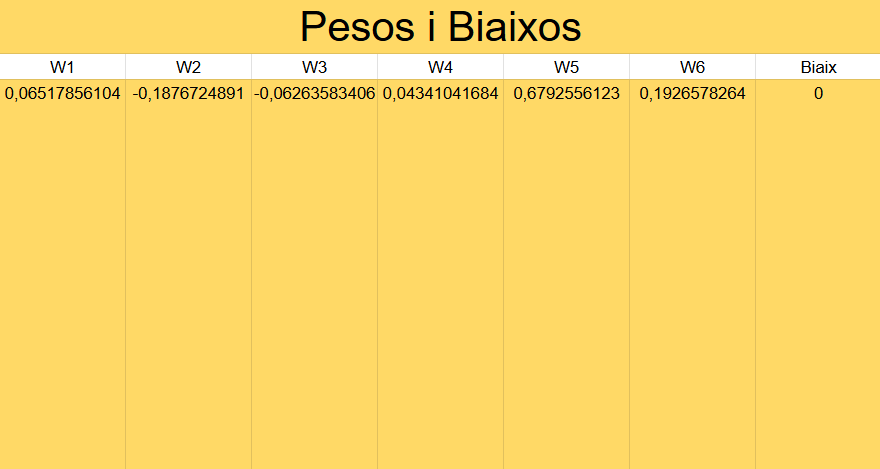
\includegraphics[width=0.5\textwidth]{./figures/Pesos_finals.png}
    \caption{Pesos finals del model}
\end{figure}

Amb aquests pesos, el model hauria de ser capaç d'obtenir unes prediccions precises respecte a la nota final dels alumnes, per obtenir els valors finals de la predicció, hem de convertir els valors normalitzats de la columna de la predicció de Y de l'última etapa en valors normals, aïllant en la mateixa fòrmula que vam emprar per normalitzar les dades.\\
$z = \frac{x - \mu}{\sigma}$\\

\begin{figure}[H]
    \centering
    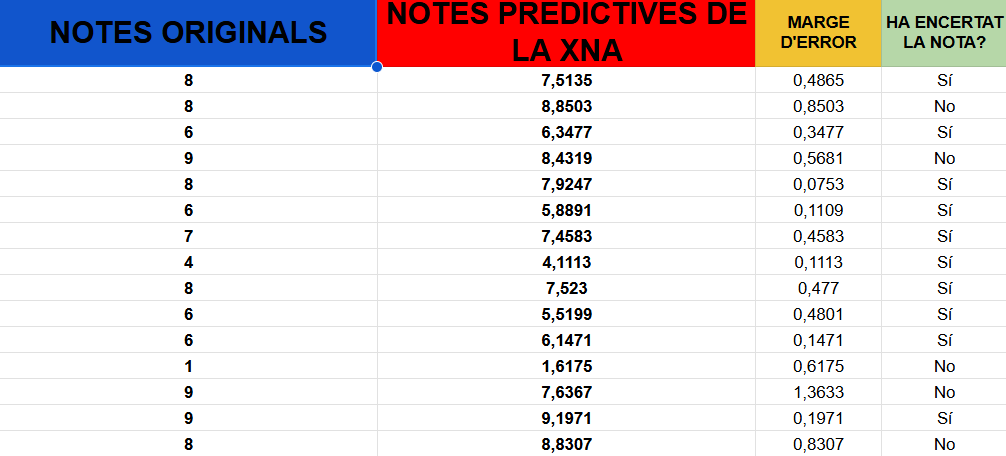
\includegraphics[width=0.5\textwidth]{./figures/Resultat_final.png}
    \caption{Prediccions finals de la pràctica}
\end{figure}

En la figura d'adalt, desprès de desnormalitzar els valors, he organitzat les notes inicials i les prediccions finals en unes taules per visualitzar-los millor, a un costat tenim les notes originals i per l'altre les predictives.

Hem de tenir en compte de que les notes finals dels alumnes estan arrodonides, per tant considerarem que la predicció ha estat encertada si té un marge d'error menor a 0,5. Això ens dona que la xarxa neuronal ha encertat 10 notes de 15, per tant té una precisió aproximada del 66,7 percent.

\section{Comparació entre una xarxa neurnal creada per un llenguatge de programació netre una de fulls de calculs}
En aquest capítol, desprès de que cadascún de nosaltras haguèssim acabat les nostres respectives pràctiques, compararem els nostres resultats finals i veurem quina de les 2 formers té més precisió.






















